\documentclass[a4paper, 12pt, openright]{book}

% language settings
\usepackage[english]{babel}
\usepackage[T1]{fontenc}

\usepackage[utf8]{inputenc}
\usepackage{textgreek}
%\usepackage{lmodern}

\usepackage{fancyhdr} % headers and footers

% figures and positioning
\usepackage{caption}
\usepackage{float}
\usepackage{graphicx}
\usepackage{graphics}
\usepackage{wrapfig}
\usepackage{listing}
%\usepackage{rotating}

% math package
\usepackage{mathtools}
\usepackage{amsthm}
\usepackage{amsmath, amssymb, dsfont, bm}

% tikz figures
\usepackage[usenames, dvipsnames, table, tikz]{xcolor}
\usepackage{tikz}
\usetikzlibrary{shapes, arrows}

% image path
\graphicspath{ {./img/} }

% add support for url and cross-references in PDF output
\usepackage{url}
\renewcommand{\UrlFont}{\color{black}\small\ttfamily}
\usepackage[colorlinks=true, linkcolor=black, citecolor=black, urlcolor=black]{hyperref}

% support for glossary and acronyms
\usepackage[acronym]{glossaries}
\newacronym[plural=MCs,firstplural=Markov Chains (MCs)]{mc}{MC}{Markov Chain}

% Costumization of theorem style
\newtheoremstyle{theoremdd}% name of the style to be used
  {\topsep}% measure of space to leave above the theorem. E.g.: 3pt
  {\topsep}% measure of space to leave below the theorem. E.g.: 3pt
  {\itshape}% name of font to use in the body of the theorem
  {0pt}% measure of space to indent
  {\bfseries}% name of head font %\color{Mahogany}
  { -- }% punctuation between head and body
  { }% space after theorem head; " " = normal interword space
  {\thmname{#1}\thmnumber{ #2}\thmnote{ (#3)}}

\theoremstyle{theoremdd}
% support for counting
\newtheorem{theorem}{Theorem}[section]
\newtheorem{corollary}{Corollary}[theorem]
\newtheorem{lemma}[theorem]{Lemma}
\newtheorem{definition}{Definition}
\newtheorem{remark}{Remark}

% added support for proof parts
\theoremstyle{remark}
\newtheorem{proofpart}{Part}
\renewcommand\theproofpart{\Roman{proofpart}}
\makeatletter
\@addtoreset{proofpart}{theorem}
\makeatother

% specific modification to basic book template of our book document
\renewcommand{\chaptername}{Section}
\addto\captionsenglish{\renewcommand{\chaptername}{Section}}
\renewcommand\qedsymbol{
\includegraphics[width=1.5cm]{occhiali}}
%\renewcommand\qedsymbol{$\square$\itshape QED}


% useful aliases for common employed declarations
\def \beq {\begin{equation}}
\def\eeq{\end{equation}}
\def\bal{\begin{align}}
\def\eal{\end{align}}
\def\prob{\ensuremath\mathbb{P}}
\def\exp{\ensuremath\mathbb{E}}
\newcommand{\Hb}{\mathbb{H}}
\newcommand{\Sb}{\mathbb{\Sigma}}
\newcommand{\U}{\mathbb{U}}
\newcommand{\F}{\mathbb{F}}
\newcommand{\V}{\mathbb{V}}
\newcommand{\A}{\mathbb{A}}
\newcommand{\B}{\mathbb{B}}
\newcommand{\C}{\mathbb{C}}
\newcommand{\E}{\mathbb{E}}
\newcommand{\I}{\mathbb{I}}
\newcommand{\Y}{\mathbb{Y}}
\newcommand{\N}{\mathbb{N}}
\newcommand{\W}{\mathbb{W}}
\newcommand{\Z}{\mathbb{Z}}
\newcommand{\R}{\mathbb{R}}
\newcommand{\X}{\mathbb{X}}
\newcommand{\Pb}{\mathbb{P}}
\newcommand{\Q}{\mathbb{Q}}
\newcommand{\D}{\mathbb{D}}
\newcommand{\Rm}{\mathbb{R^{-1}}}
\newcommand{\J}{\mathbb{J}}

\newcommand{\Fig}[1]{Fig.~\ref{#1}}
\newcommand{\eq}[1]{(\ref{#1})}
\newcommand{\Tab}[1]{Tab.~\ref{#1}}
\newcommand{\Sec}[1]{Sec.~\ref{#1}}
\newcommand{\indep}{\mathrel{\perp\mspace{-10mu}\perp}}
\newcommand{\RN}[1]{ \textup{\uppercase\expandafter{\romannumeral#1}}}

\begin{document}
\section{Elementary renewal theorem}
Let's take the limit
\beq
\lim_{t \to \infty}\frac{M(t)}{t} = \frac{1}{\mu}
\eeq
where $\mu = E[X]$.\\
Then we can prove that $\frac{M(t)}{t} = E[\frac{N(t)}{t}]$ and that $\lim_{t \to \infty}\frac{M(t)}{t} = \frac{1}{\mu}$ w.p. 1.
\subsubsection{Counter example} 
Let $U$ be a uniform r.v. $U(0,1)$ and let $Y_n$ be a r.v. such that:
\beq
Y_n =
\begin{cases}
0 \quad for \quad U \ > \frac{1}{n}\\
n \quad for \quad U \leq \frac{1}{n}
\end{cases}
\eeq
Where the second equation brings to the espressions $\frac{M(t)}{t} > \frac{1}{\mu} - \frac{1}{t}$ and $\lim_{t \to \infty} \frac{M(t)}{t} \geq \frac{1}{\mu}$

\textbf{NOTE}: In the book the notation has also the expression \textit{"lim \textbf{inf}"} since, in this way, the demonstration is "easier" to do, in fact we can also see graphically that the $inf$ expression guarantees that we have a lower bound. Figure\ref{fig:graph1}
\begin{figure}[h]
\centering
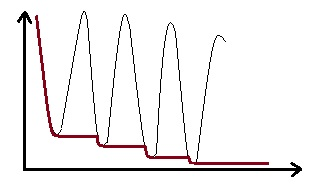
\includegraphics[width=0.5\textwidth]{Cri_graph1.jpg}
\caption{lower bound}
\label{fig:graph1}
\end{figure}
Now the other bound must be proved, so to reach the equality, but here there is a problem: $S_{N(t)}$ is not known, so it is difficult to demonstrate the inequality $t \geq S_{N(t)}$ since I cannot take the expectation. So we use a \textbf{trick}: we consider a new renewal process obtained by the previous one by truncation:
\begin{equation}
X_i^c =
\begin{cases}
X_i \qquad X_i \leq c\\
c \qquad X_i >c
\end{cases}
\end{equation}

What do we have for this truncated process?\\
First of all we have the relations:
\begin{equation}
\begin{split}
N^c(t) \geq N(t)\\
M^c(t) \geq M(t)
\end{split}
\end{equation}
because, since events are spaced by numbers that are no bigger, times are no smaller.\\

So for the truncated process we have $t \geq S_{N^c(t) +1}$ (in the truncated process, the $X$ I'm adding cannot be bigger than $c$), and the next inequality also goes:
\begin{equation}
c+t \geq S_{N^c(t)+1}
\end{equation}•
If now I take this inequality expectation I obtain:
\begin{equation}
t+c \geq \mu^c(1+M^c(t))
\end{equation}•
and since $M^c(t) \geq M(t)$ from the previous inequality, I can say that:
\begin{align}
\begin{split}
\mu^c(1+M^c(t)) \geq \mu^c(1+M(t))\\
\frac{M(t)}{t} \leq \frac{1}{\mu^c} \frac{1}{t}(\frac{c}{\mu^c}-1) \qquad \forall c > 0 \quad (valid\quad for\quad any\quad truncation)
\end{split}
\end{align}

NOTE: $c$ is an index, not an exponent.
So now I take the limit:
\beq
\lim_{t \to \infty} sup \frac{M(t)}{t} \leq \frac{1}{\mu^c} \qquad \forall c > 0
\eeq
Since it is true $\forall c$ , it is true also for $c \to \infty$ (which means that truncation becomes less an less important until I don't truncate at all), so I obtain:
\beq
\lim_{t \to \infty} sup \frac{M(t)}{t} \leq \lim_{c \to \infty} \frac{1}{\mu^c}
\eeq
where $\mu^c = \int_0^c(1-F(x))\,dx$, so as $c \to \infty$ we see that $\mu^c \to \mu = \int_0^\infty(1-F(x))\,dx$. See figure\ref{fig:mu}
\begin{figure}
\centering
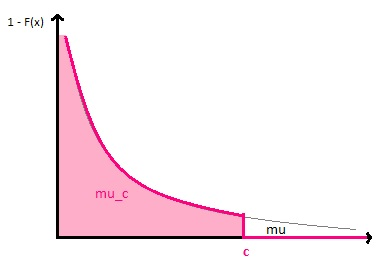
\includegraphics[width = 0.5\textwidth]{Cri_mu.jpg}
\caption{This graph is the complementary distribution of $X^c$}
\label{fig:mu}
\end{figure}
So at the end we conclude that
\beq
\lim_{t \to \infty} sup \frac{M(t)}{t} \leq \lim_{c \to \infty} \frac{1}{\mu^c} = \frac{1}{\mu}
\eeq
\\
\textit{cvd}
\subsection*{Observation}
In the book, at the beginning, they assume that $E[X] < \infty$. Reasoning on it we can observe that:
\begin{itemize}
\item In the first part is not needed;
\item In the second one, even though $\mu = 0$, I can make it finite by truncation;
\end{itemize}
\subsection{Two important results proofs}
We now proceed with proving two important results:
\begin{itemize}
\item \textbf{1}: $E[S_{N(t)+1}] = (1+M(t))E[X]$;
\item \textbf{2}: $E[S_{N(t)}] \ne M(t)E[X]$;
\end{itemize}
In the first case there is no case in which the equality is not true, so we can state that this equality is always true; in the second case there is a non-zero number of cases in which the equality is not true, and so it cannot taken as true in general.
\subsubsection*{$1^{st}$ Statement}
In this case represents a Poisson process: $S_{N(t)+1} = t + \gamma_t$ and $S_{N(t)} = t - \delta_t$;\\
If i sit at time $t$, then $\gamma_t$ is the time until the next renewal, which means that the time until the next renewal occurs is $t + \gamma_t$, and so this is why $S_{N(t)}$ is the instant $t$ minus the time since the last renewal occurred $\delta_t$. And that's actually true for any renewal process.\\
Moreover we know that both $\gamma$ and $\delta$ are exponentially distributed (because of Poisson process theory and the memoryless condition of the process): $\gamma_t$ is exponential with parameter $\lambda$, while $\delta_t$ is exponential with parameter $\lambda$ truncated at $t$.\\
So we can find all the quantities involved:%min 25:00
\beq
E[S_{N(t)+1} = t + \frac{1}{\lambda}] \qquad E[S_{N(t)}] = t - \frac{1-e^{-\lambda t}}{\lambda}
\eeq
with $M(t) = \lambda t$ and $E[X] = \frac{1}{\lambda}$.\\
Thanks to it we can see that the equality in true.
\subsubsection*{$2^{nd}$ Statement}
In this case we take:
\beq
X_i =
\begin{cases}
1 \qquad w.p. p\\
a \geq 2 \qquad w.p. 1-p
\end{cases}
\eeq
How many arrivals do we count?
\beq
N(t) = 
\begin{cases}
1 \qquad w.p. p\\
0 \qquad w.p. 1-p
\end{cases}
\eeq
And how much time do we count?
\beq
S_{N(t)}=
\begin{cases}
1 \qquad w.p. p\\
0 \qquad w.p. 1-p
\end{cases}
\eeq
NOTE: Even though the value is the same, they do not represent the same thing.\\
What about $S_{N(t)+1}$? $a>t$ so:
\beq
S_{N(t)+1} =
\begin{cases}
a \quad \text{w.p. $ (1-p)$}  \rightarrow \text{it means it the first renewal}\\
2  \quad \text{w.p.  $p^2$}  \rightarrow \text{if the first  X is 1 and also the second}\\
1+a \quad \text{w.p. $ p(1-p)$} \rightarrow \text{if the first X is 1 and the second is a}\\
\end{cases}
\eeq
So:
\beq
\begin{split}
E[S_{N(t)+1}] & = a(1-p)+2p^2+(1+a)p(1-p)\\
                        & = p^2 + p + (1-p^2)a\\
\end{split}
\eeq
\beq
\begin{split}
E[S_{N(t)}] & = p\cdot1 + 0\cdot(1-p)\\
	         & = p E[N(t)] = M(t)\\
	         & =  p\cdot1 + (1-p)\cdot0 = p
\end{split}
\eeq
So I can try those equalities by multiplying
\beq
E[N(t)+1]E[X] = (1+p)(p+a(1-p)) = p^2+p+(1-p^2)a = E[S_{N(t)+1}]
\eeq
On the other hand:
\beq
E[N(t)]E[X] = p(p+(1-p)a) \ne p
\eeq
$\leftarrow$ {I can always find a value of $a$ that makes the equality not true}
So the first equation was found to be true in both cases and it's contrary for the second.
\subsection{Exercises}
\subsubsection*{Ex 2.4}
Each specific error is found on a specific case w.p. $\frac{1}{600}$ so the number of errors on given page is a binomial r.v. $(240,\frac{1}{600})$. At the same time, though, we know that when we have a Bin where $p$ is small and $M$ is big we can approximate it to a Poisson r.v. $\sim P(\frac{240}{600})$, where $\lambda = \frac{240}{600}  \simeq 0.4$.\\
So I represent the book as:
\begin{figure}[h]
\centering
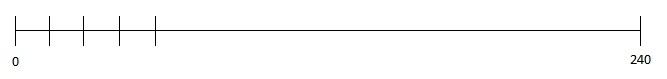
\includegraphics[width = 0.6\textwidth]{Cri_book.jpg}
\label{fig:book}
\end{figure}
Easy to find the probability of what happens i different pages: each page is an independent interval, so:
\beq
P[\text{0 errors in 3 pages}\footnote{not necessarily consecutive}] = e^{-1.2}
\eeq
\subsubsection*{Ex 2.5}
We have $N$ points equally distributed in a circle of radius $r$. The distribution of points in the circle of radius $1$ as $N \to \infty$ and $r \to \infty$ is:
\beq
\frac{N}{\pi r^2} < \lambda
\eeq
While the probability \textit{Prob[points inside r = 1]} is:
\beq
\frac{Small_{Area}}{Big_{Area}}
\eeq
This bring us to say that \textit{P[a given point is inside r $\leq$ 1] = } $\frac{Area(1)}{Area(r)} = \frac{1}{r^2}$.\\
The number of points present in the smaller circle is a binary r.v. $\sim bin(N,\frac{1}{r^2})$, so its expected value is:
\beq
\text{E[number of points inside the smaller circle]} = \frac{N}{r^2} = \lambda\pi
\eeq
where $\lambda$ is the density of points and $\pi$ is the area of unitary circle.\\
So we have two parameters, the product of which is still constant.
\begin{align}
\begin{split}
N \to \infty \qquad r \to \infty\\
\frac{N}{\pi r^2} = \lambda' \rightarrow P_{0i}(\lambda\pi)
\end{split}
\end{align}
\subsubsection*{Ex 3.6}
For $i = 1 \dots n$ I have an indep. PP $\rightarrow X_i(t)$ is an i.i.d. PP($\lambda$).\\
The problem asks to find the first time such that there is at least one event  in every process, see figure\ref{fig:3.6}
\begin{figure}[h]
\centering
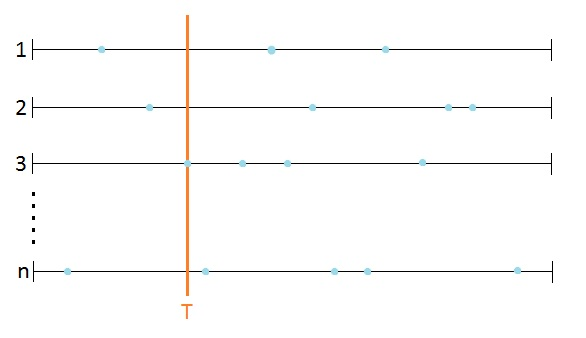
\includegraphics[width =0.6\textwidth]{Cri_Ex3_6.jpg}
\label{3.6}
\end{figure}
Since the process is Poisson, we have that $P[T\leq t] = 1-P[0 events] = 1-e^{-\lambda t}$ for one process, while for $n$ processes we have $P[t \leq t] = (1-e^{}-\lambda t)^n$.\\
We could actually see the problem from a different point of view: this view counts the events in the Poisson Poisson process and uses the independence to find the probability that none of them has seen $0$ events.\\
So we can see how we can look at $T$: we get that $T$ is the time at which the last process has its first event and it will be the biggest value among the exponentials; the first event will occur, obviously, with exponential time, so using this reasoning we can express the r.v. $T$ as:
\beq
T = \max_{i = 1,2,\dots,n}{exp_i(\lambda)}
\eeq
So I can turn the point into a question: what is the distribution of the maximum among the i.i.d variables? 
\begin{align}
\begin{split}
P[max{X_1,X_2,\dots,X_n} \leq t] & = P[X_i \leq t, \quad i = 1,2, \dots, n]\footnote{since the X's are i.i.d.}\\
					  & = (P[X \leq t])^n = (1-e^{-\lambda t})^n
\end{split}
\end{align}
In general this shows that if we take $F_{max}(t)$, then $F_{max}(t) = (F(t))^n$; on the other side:
\begin{align}
\begin{split}
P[min{X_1,X_2,\dots,X_n} >t ] & = P[X_i > t \forall i = 1,2,\dots, n] \\
				        & = (P[X > t])^n
\end{split}
\end{align}
So we found that $1-F_{min}(t) = (1-F(t))^n \rightarrow F_{min}(t) = 1- (1-F(t))^n$
\subsubsection*{Problem 3.6}
Service facility situation: service when $Q$ users arrived $\rightarrow$ a process that focuses on the $q^{th}$ arrival in sequence.\\
$T = $ service time.
\begin{figure}
\centering
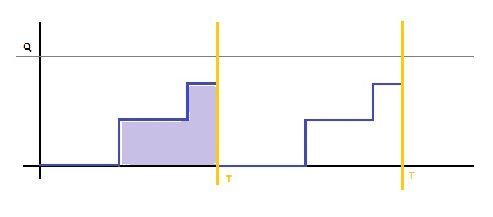
\includegraphics[width = 0.6\textwidth]{Cri_scale.jpg}
\caption{Prob 3.6}
\end{figure}
We have to show that $E[\int_{0}^{T}N(t)dt] = \frac{q(Q-1)}{2\lambda}$; The first question is intuitive: we can see that if the time at which a user is served is the time at which the $q^{th}$ user arrives, then I have to wait for $q$ users to arrive to be served.\\
I then have to take the expectation of the blue area, to do it I can use two different approaches: I can look how much time each user has to wait and then I sum all of then (and that corresponds to summing the horizontal slices of the area), or I can look at it vertically and see how much time there is one, two, three users waiting and then multiplying this amount of time by the number of users who are waiting during that time.\\
So with the first approach:
\begin{itemize}
\item The first user will have to wait $\frac{1}{\lambda}(Q-1)$ inter-arrival times;
\item The second user arrives after $2$ inter-arrival times and so he has to wait $\frac{1}{\lambda }(Q-2)$ inter-arrival times; 
\item After the second user more users will arrive until the $q^{th}$ user will arrive, and for it the waiting time will be $0$;
\end{itemize}
So the average sum of all the waiting time is the constant $1/\lambda$ times  the sum of the first $Q-1$ integers: $\frac{1}{\lambda}[(Q-1)+(Q-2)+\dots+1]$.\\
With the second approach we see that:
\begin{itemize}
\item At the beginning no one is waiting in line;
\item After the first arrival $1$ user is waiting;
\item After the second arrival $2$ users are waiting;
\item After the $(q)^{th}$ arrival, $Q-1$ users are waiting and so the structure is the same as previously.
\end{itemize}
\subsubsection*{Ex 4.1}
Given $n$ arrivals, we take the quantity $E[w_1] = \int_{0}^{1}(1-t)^n dt = \frac{1}{n+1}$ where $w_1$ is the smallest among $n$ i.i.d. uniform r.v. between $0$ and $1$ and so the distribution is the distribution of the minimum of $n$ i.i.d. uniform r.v., and its complementary distribution is the $n^{th}$ power of the complementary distribution.\\
\subsubsection*{Ex 4.3}
Suppose we have $5$ arrivals, the cumulative time is the area in figure4, but we know that the arrival times are i.i.d. uniform so each user has to wait average waiting time is $0.5$ hours, so $0.5\times5 = 2.5$.\\
\subsubsection*{Ex 4.5}
Here assume we have $\alpha$  and the service time is an exponential r.v. $\sim exp(\alpha)$, and the probability $P[\text{at time 1 h the queue is empty}]$ is estimated considering each user arriving uniformly. So at the end the number of users is binomial and, conditioning on the uniform variable, we get:
\begin{align}
\begin{split}
p = P & [\text{a uniformly arriving user has not left at time 1 h}] =\\
& P[U_i + Y_i > 1] = \int_{0}^{1}e^{-\alpha(1-u)}du = \frac{1-e^{-\alpha}}{\alpha}
\end{split}
\end{align}
So the probability becomes finding the probability that all users that had arrived here have left: it is the value $(1-P)^{n}$ with $n = $ \textit{number of users}:
\begin{align}
P&[\text{System empty at time 1|5 arrivals}] = (1-\frac{1-e^{-\alpha}}{\alpha})^5
\end{align}
\begin{figure}[h]
\begin{minipage}[c]{0.5\textwidth}
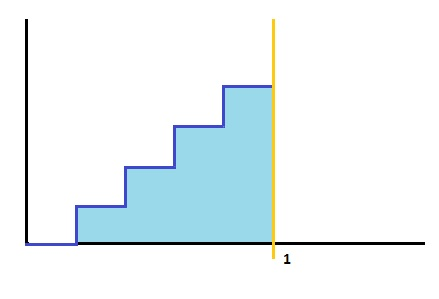
\includegraphics[width = 0.9\textwidth]{Cri_area.jpg}
\caption{Ex 4.3}
\end{minipage}
\hspace{10mm}
\label{fig:area}
\begin{minipage}[c]{0.5\textwidth}
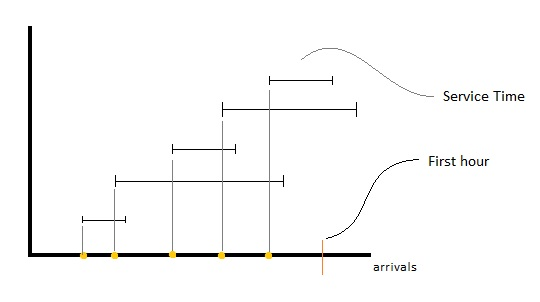
\includegraphics[width = 0.9\textwidth]{Cri_arrivals.jpg}
\caption{Ex 4.5}
\end{minipage}
\end{figure}
\end{document}





















